% EXAMPLE: Sections and Paragraphs
% \section		- Level 1
% \subsection		- Level 2
% \subsubsection	- Level 3
% \paragraph		- Level 4
% \subparagraph		- Level 5 
% \section{<NAME_OF_SECTION>}

% EXAMPLE: Include graphics 
% \includegraphics[width=130mm,height=108mm]{intro4.png}

% EXAMPLE: Nested list
%\begin{enumerate}
%\item Nested list
%\begin{enumerate}
%\item
%\item
%\item
%\item
%\item
%\end{enumerate}
%\end{enumerate}
\section{Appendix A - How to build upon the codebase}
This appendix include information on how to build upon our codebase for the Mulle (C), server code (Python, PHP/HTML5 and C) and Android Mobile phone (Java).
\subsection{Mulle}
The Mulle communication via COAP is far from finished and therefore here is a guide how to get started followed by what should be further built. The instruction on how to get started are done in Ubuntu, the versions that were tested are 10.04 and 11.10. Windows or any other OS will not be covered in this guide.

The Mulle software required is all in the Software-PAN-NAP folder which contain necessary libraries and applications. It is assumed that you have acquired this because it's essential for any development.

\subsubsection{Getting started}
The first step you will take is to download the code from a repository on Github.com, if you don't know how to do this there are several guides how to do that on their site. Since there are several ways to do this here are the links to the repository:
\begin{itemize}
\item Download zip: \url{https://github.com/christofferholmstedt/vehicletesting/zipball/master}
\item Git: \url{git://github.com/christofferholmstedt/vehicletesting.git}
\item SSH: \url{git@github.com:christofferholmstedt/vehicletesting.git}
\end{itemize}
When you've done this note that you'll only need files from the ../vehicletesting/code/Mulle folder.
In this folder there are two subfolders named Coap and PAN-Router\_demo. 
These two folders are going to seperate locations in your Mulle software folder, 
since the Coap folder contains the code for the protocol and PAN-Router\_demo code for the application. 

The folder Coap should be copied into ../$<$Mulle Software folder$>$/Libary/misc/apps/ 
and the PAN-Router\_demo folder goes to  ../$<$Mulle Software folder$>$/Applications/. 
The PAN-Router\_demo folder is optional to use, if you want to use you're own Mulle program you need to include coap.h and run coap\_init() somewhere in your applications c-file. 
Since the coap-protocol isn't official you also need to put a "\#define LWIP\_COAP" and set it to 1 in proj\_arch.h(as well as turn off any other protocol that are used for communcation) 
and finally you need to add coap.c in the SOURCES.mk file. This is done by adding "\$(LIBDIR)/misc/apps/coap/coap.c" to the LWIP\_Apps field.

Now when you have the code set up you must install the gcc compiler, namely m32c-elf-gcc, for this type of hardware. Do the following steps in your terminal with sudo, alternatively make a script. Be prepared to redo this if you're doing it in a script. It's preferable to do this step by step because it has a higher rate of succeeding. 

Alternatively you can follow this guide(however, it's strongly advised not to): \url{http://www.eistec.se/docs/wiki/index.php?title=Mulle\_software\_with\_GCC}

Setup Development Host:
\begin{itemize}
\item apt-get install build-essential
\item apt-get install m4 autoconf libtool gawk bzip2 bison flex gettext texinfo zlib1g-dev 
\item apt-get install libmpc-dev libmpfr-dev
\end{itemize}

\noindent When this is done you need to download binutils and install it:
\begin{itemize}
\item wget \url{http://ftp.gnu.org/gnu/binutils/binutils-2.19.1.tar.bz2}
\item tar xjf binutils-2.19.1.tar.bz2
\item mkdir binutils-obj
\item cd binutils-obj
\item ../binutils-2.19.1/configure --target=m32c-elf
\item make
\item sudo make install
\item cd ..
\end{itemize}

\noindent In the next step you'll download gcc-4.3.3 and newlib 1.17 and install them:
\begin{itemize}
\item wget \url{ftp://ftp.nluug.nl/mirror/languages/gcc/releases/gcc-4.3.3/gcc-4.3.3.tar.bz2}
\item wget \url{ftp://ftp.nluug.nl/mirror/languages/gcc/releases/gcc-4.3.3/gcc-core-4.3.3.tar.bz2}
\item wget \url{ftp://sources.redhat.com/pub/newlib/newlib-1.17.0.tar.gz}
\item tar xjf gcc-4.3.3.tar.bz2
\item tar xjf gcc-core-4.3.3.tar.bz2
\item tar xzf newlib-1.17.0.tar.gz
\item cd gcc-4.3.3
\item ln -s ../newlib-1.17.0/newlib
\item ln -s ../newlib-1.17.0/libgloss
\item cd ..
\item mkdir gcc-obj
\item cd gcc-obj
\item ../gcc-4.3.3/configure --target=m32c-elf --with-newlib --enable-languages="c"
\item make
\item sudo make install
\item cd ..
\end{itemize}
When you've done all these steps you should try typing this into your terminal: "m32c-elf-gcc --version" and check that it says "m32c-elf-gcc (GCC) 4.3.3" just to be sure.

Now you're good to go, a final note on how get get set up is how to push your code onto the Mulle. Pushing your programs is done in a few steps, first you need to orient your way to the folder containing the program you're pushing in the terminal, then do these steps:
\begin{itemize}
\item make clean
\item make all
\item make program
\item make debug
\end{itemize}
The “make clean” is only needed if you changed something in the system files and when running “make program” the Mulle must be set to “Program Mode”. If all your modified files are correct your code will be pushed to the Mulle, if you get a “Clock Validation Error” make sure the Mulle is set to “Program Mode” and try again. The “make debug” command starts mulle\_term, which is a terminal debugger for the Mulle, so when you put it back on “Run Mode” you'll see what it is doing(in the form of printouts).

\subsubsection{Further developement}

You will need some sort of device that can share internet through Bluetooth to the Mulle, whether it be a telephone or a personal computer with an USB-dongle. To test COAP protocol, you can download the Copper addon for Firefox. The coap\_init() function in coap.c initializes so that when you receive UDP packets on the Mulle the function coap\_input() is run.

First the coap\_input() function needs to be properly made, since it does nothing useful at this time. What needs to be done is that the function should put all the correct values into a coap struct and based on what values are in each field the function should decide where to send the infomation next for handing. 

A suggestion for handling the COAP payload is by working with EXIP. You create and decode exi files directly on the mulle. EXI-files which have the same structure as XML are interesting for this type of projects since it's light and you can easily write scripts with XML structure.

You can find out more about EXIP here: http://exip.sourceforge.net/ .
A final suggestion is to finish the debug\_coap\_print() function since it will be very helpful for debugging.

\subsection{Server}
\subsubsection{Coapy server}
\paragraph{Existing implementation}
The server is based on CoAPy, which is a python implementation of the CoAP protocol. The actual server implementation is a modification of the example server provided along with CoAPy.
Some minor changes were made to it allowing it to accept all forms of CoAP messages, provided they are taken care of properly. We also added a way for new services to be easily added 
and used. 

The procedure when adding new services is as follows:
\begin{enumerate}
\item Create a new .py file with the name corresponding to the actual service name (e.g. "TestService.py") in the "services" directory
\item The file should contain only the necessary imports (including CoAPy parts) along with a class name the same thing as the file ("TestService", in this case)
\item The class is to define a single function "process" in which the actual actions of the service are to be made
\end{enumerate}

Using an existing service, like "CounterService.py", is highly recommended for understanding how a service should be structured and laid out.

\paragraph{Further development}
The server itself should be set to add new services for operation. What needs more work is the incorporation of a few things:

\begin{enumerate}
\item An actual XML scheme for configuration of mulle nodes. This point is not particular to the server, however.
\item Implement ways for the server to make use of the EXIP application to translate the XML that's to be sent into EXI via the command line.
\item Make services corresponding to the functionality you would like to have for configuration and communication with mulles and android devices, respectively.
\end{enumerate}
\subsubsection{Webpages and database}
 
The webpages and database consists of Apache2 which is an web server, MySQL which is a database management system and PHP which is a language for producing dynamic webpages.
LAMP (Linux), WAMP (Windows) or MAMP (Mac) can be used to build a web server it is an web-platform that consists of Apache, MySQL and PHP.

\paragraph{Webpages}

The webpages are built up using mulleheader.php which contains the header and sidebar, a .php file containing page content and mullefooter.php which contains the footer.

We have built two webpages using this concept; One that shows information from the database and its .php file that holds page content is mulledatabase.php and one consists of 
a php form to turn on or off a lamp and its .php file that holds page content is mullebuttons.php. The mullebuttons.php also contains a call to a .py file called testsender.py
that with some work can run a service on the CoAP server.


How to create a new webpage:

1. 	Create a new .php file for page content

2. 	In the top of the .php file print:\\$<?$php include("mulleheader.php"); $?>$

3. 	Between \\$<$ section id ="main" $>$ and $<$/section $>$ write the page content

4. 	In the bottom of the .php file print \\$<?$php include("mullefooter.php"); $?>$

\paragraph{Database}

We created a MySQL database and named it mulle and to this database we added two tables one that keeps track of communication on server and one that keeps track of connected/active 
devices. Online you can find many guides on how to add to a LAMP, WAMP or MAPM MySQL database, but down below shows some commands good to know when creating a database.  


How to create a new database:

1. 	Open up your MySQL Console and login

2. 	mysql$>$ \texttt{SHOW DATABASES;}

3. 	mysql$>$ \texttt{CREATE DATABASE the_database_name;}

4. 	mysql$>$ \texttt{USE the_database_name}

5. 	\texttt{CREATE TABLE name_of_table (name_first_column_in_table VARCHAR(20), name_second_column_in_table VARCHAR(20), name_date_and_time DATETIME);}
	This creates a table with three columns.
	
6. 	\texttt{SHOW TABLES;}

7. 	\texttt{EXPLAIN name_of_table;}

\subsection{Android Mobile Phone application}

The primary goals for the android applications were to;
%communication goes via a server.
\begin{itemize}
 \item communicate using CoAP over an UDP connection
 \item encode the sent packets with EXI to reduce the size of packets
 \item have a graphical UI capable of controlling multiple devices.
\end{itemize}
% UNDERSÖK OM MER SKA IN HÄR

\subsubsection{The finished product}

The application starts off by showing the server menu. One will have to either add a server or use a saved one. 
Clicking on a server in the list will cause the application to validate that the server is alive and thereafter it will perform a CoAP discovery on the server. 
When receiving an answer to the discovery the application will start filling the device menu with devices and their services. The device menu can then be accessed to use the services available.
The services generally works as follows: The application gets a click on the chosen service, so it sends it message to the service owner, whereafter the service owner either changes something or responds.
The device will then have to respond to the application with the updates made, this can be with a confirmation or a whole new CoAP message. This makes the application respond by updating the GUI with the new values.

The pre-built services are generalized to: 
\begin{itemize}
 \item IsOn, provides an item with a checkbox that is checked if a service is on (for example a lamp). Clicking on this should provide a change on the selected device.
 \item GetValue, provides an item which shows the last value provided. Clicking on the item should provide an update.
 \item SendValue, provides an item which have a textbox where one can send a payload to the device. %ska denna även visa vad värdet är för tillfället? tror det 
\end{itemize}

Another planned feature is the options menu where the application will allow things like turning EXI encoding on or off. 

\subsubsection{What exists today}

Today there exists a communication part which allows one to send and recieve CoAP messages. This part uses a library made out of \texttt{jCoAP revision 202b8f8eb7b4, http://code.google.com/p/jcoap/}%s.unger.mobil@gmail.com committer ,	chr.lerche@gmail.com	owner,	nic@nclm.de	owner
 to get the CoAP features. This part is not yet a completed project but the features requested for this application is present. The EXI converter is currently not available but is planned to use exificient, 
which can be found at \url{http://exificient.sourceforge.net/}.

The GUI is another important part of the application. It is built to be able to controll multiple servers and devices. 
To make this possible the application has 3 tabs:	%the default thought was to have a checkbox in the server menu to allow one to decide whether a server is being currently used, this idea has however been dropped due to lack of time.
\begin{itemize}
 \item Device tab
 \item Server tab
 \item Options tab
\end{itemize}

The Options tab does currently not contain anything but should simply allow a user to change things about how the application should work and what and how things should be displayed. 

 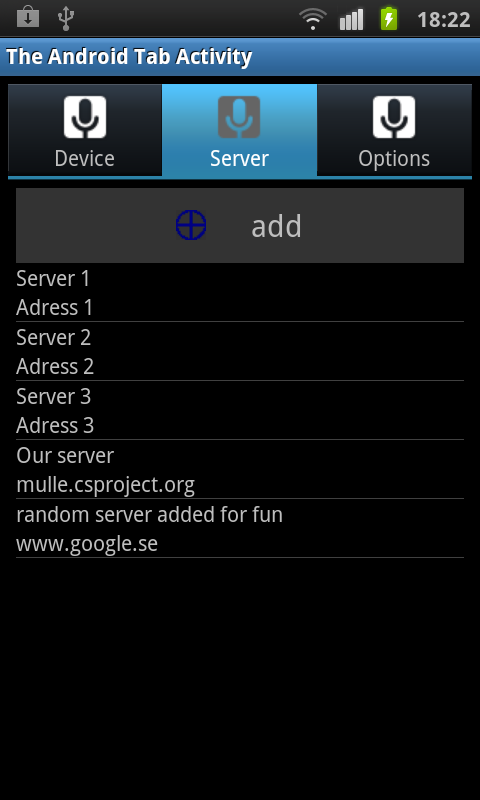
\includegraphics[scale=0.50]{android-server.png}%\caption{The Server tab of the Android application}
\\The Server tab shows all the active servers. You can click on the add button in the server menu and a window appears where you write in the name and the adress. The servers then appears in a listview where it's easy to keep track of them.
In the future this can be complemented with a network discovery of nodes, however, my personal opinion is that it should be possible to manually add an server.

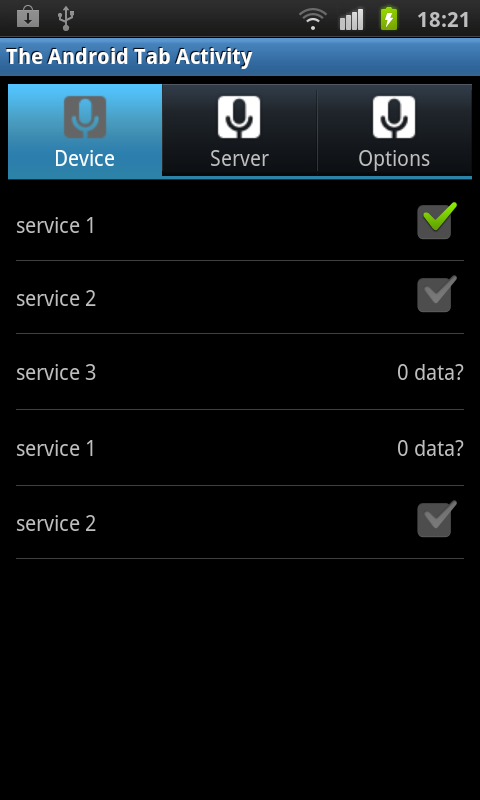
\includegraphics[scale=0.50]{android-device.png}%\caption{The device tab of the Android application}
\\The Device tab is the latest addition in the GUI and contains the actual services that are available. It contains a custom ArrayAdapter that have been tweaked to be able to display children of the interface rowdata.
In it's current state it is possible to add items to this list in the code by calling the NewItem() function with proper parameters. Adding service types if the pre-built service types are not enough is easy. 
Simply extend the rowdata() interface and create the desired xml for the item, do not however forget to add a typenumber for the NewItem() function to be able to create it. 
This also allows the children to define for their own what should happen if clicked, updated and so on.






